\begin{frame}{Custom Tick Marks}
\begin{center}
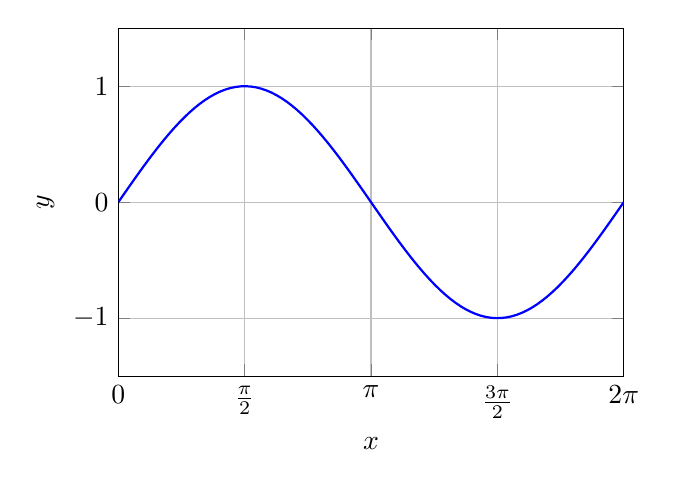
\begin{tikzpicture}
\begin{axis}[
    xlabel={$x$},
    ylabel={$y$},
    grid=both,
    xmin=0, xmax=2*pi,
    ymin=-1.5, ymax=1.5,
    width=8cm,
    height=6cm,
    xtick={0,pi/2,pi,3*pi/2,2*pi},
    xticklabels={0,$\frac{\pi}{2}$,$\pi$,$\frac{3\pi}{2}$,$2\pi$},
    ytick={-1,0,1}
]
\addplot[thick, blue, domain=0:2*pi, samples=100] {sin(deg(x))};
\end{axis}
\end{tikzpicture}
\end{center}

\footnotesize
\texttt{xtick=\{0,pi/2,pi,3*pi/2,2*pi\},}\\
\texttt{xticklabels=\{0,\$\textbackslash frac\{\textbackslash pi\}\{2\}\$,\$\textbackslash pi\$,\$\textbackslash frac\{3\textbackslash pi\}\{2\}\$,\$2\textbackslash pi\$\}}
\end{frame}